\documentclass[12pt, a4paper]{article}
\usepackage[utf8]{inputenc}
\usepackage[spanish]{babel}
\usepackage{geometry}
\geometry{margin=2.5cm}
\usepackage{setspace}
\usepackage{booktabs}
\usepackage{array}
\usepackage{graphicx}
\usepackage{url}
\usepackage{hyperref}
\hypersetup{colorlinks=true, linkcolor=black, urlcolor=black, citecolor=black}
\usepackage{amsmath}
\usepackage{float}
\onehalfspacing

\graphicspath{{./Regresion/paper/figuras/}}

\title{\textbf{Predicción de Costos de Seguro Médico Mediante\\
Modelos de Regresión y Aprendizaje Automático}\\[6pt]
\large Ingeniería de Features, Comparación de Seis Modelos y Despliegue Web}

\author{Juan David Peralta Fuentes\\
\small Electiva V -- Ciencia de Datos\\
\small Docente: Aimer J. Rivera Centeno\\
\small Universidad Popular del Cesar\\
\small Facultad de Ingenierías y Tecnología\\
\small \texttt{jdavidperalta@unicesar.edu.co}}
\date{Abril 2026}

\begin{document}

\maketitle

% ── ABSTRACT ──────────────────────────────────────────────────
\begin{abstract}
La predicción de costos de seguros médicos es un problema de alto impacto
económico para aseguradoras y sistemas de salud. Este trabajo aplica
regresión supervisada sobre el \textit{Medical Cost Personal Dataset}
de Kaggle, que contiene 1.338 registros con características demográficas
y de salud. Siguiendo la metodología CRISP-DM, se entrenaron y compararon
seis modelos: Regresión Lineal, Ridge, Lasso, Random Forest, XGBoost y
Gradient Boosting. Se incorporaron interacciones no lineales
(BMI $\times$ tabaquismo, edad$^2$) como ingeniería de features para
capturar relaciones no capturables por modelos lineales. El mejor modelo
alcanzó un $R^2$ de \textbf{0.8730} y un MAE de \textbf{\$2,495.65},
superando al baseline lineal en \textbf{0.6}\,\%. Los resultados
confirman el tabaquismo como el factor predictor más determinante del
costo anual del seguro.
\end{abstract}

\noindent\textbf{Palabras clave:} regresión, XGBoost, Random Forest,
seguro médico, predicción de costos, ingeniería de features, CRISP-DM,
tabaquismo, BMI.

\tableofcontents
\newpage

% ══════════════════════════════════════════════════════════════
\section{Introducción}
% ══════════════════════════════════════════════════════════════

El gasto en salud representa uno de los principales desafíos financieros
para individuos y sistemas de cobertura médica. En Estados Unidos, el gasto
per cápita en salud superó los \$12.500 dólares anuales en 2020,
representando el 19{,}7\,\% del PIB \cite{cms2022national}. La capacidad
de predecir con precisión los costos médicos individuales permite a las
aseguradoras fijar primas justas, gestionar riesgos y diseñar programas
de prevención dirigidos.

Los modelos de regresión supervisada han demostrado ser herramientas
eficaces para la predicción de costos médicos, capturando tanto relaciones
lineales como interacciones complejas entre variables demográficas y
factores de riesgo \cite{duan2021prediction}. Sin embargo, la efectividad
de estos modelos depende fuertemente de la calidad del preprocesamiento y
la ingeniería de features aplicada.

El principal reto estadístico de este dataset es la \textbf{asimetría
positiva} de la variable objetivo \texttt{charges}: su distribución
presenta una cola derecha larga con unos pocos individuos de costos muy
elevados, típica de datos de gastos en salud. Esta asimetría reduce el
rendimiento de los modelos lineales y motiva el uso de transformaciones
y modelos basados en árboles.

El objetivo de este trabajo es comparar seis modelos de regresión bajo
la metodología CRISP-DM, evaluar el impacto de la ingeniería de features
en el rendimiento predictivo e identificar los factores más influyentes
en el costo del seguro.

% ══════════════════════════════════════════════════════════════
\section{Descripción del Dataset}
% ══════════════════════════════════════════════════════════════

El \textit{Medical Cost Personal Dataset} fue obtenido de Kaggle
\cite{insuranceKaggle} y contiene 1.338 registros de asegurados de
Estados Unidos. No presenta valores nulos en ninguna columna.

\begin{table}[H]
\centering
\caption{Variables del Medical Cost Personal Dataset}
\small
\begin{tabular}{>{\bfseries}p{3.5cm} p{2.2cm} p{7cm}}
\toprule
Variable & Tipo & Descripción \\
\midrule
age      & Numérica   & Edad del asegurado principal en años \\
sex      & Categórica & Género: \texttt{male} / \texttt{female} \\
bmi      & Numérica   & Índice de Masa Corporal en kg/m² \\
children & Numérica   & Número de hijos dependientes cubiertos \\
smoker   & Categórica & Estatus fumador: \texttt{yes} / \texttt{no} \\
region   & Categórica & Región de EE.UU.: \texttt{southwest, southeast,}
                         \texttt{northwest, northeast} \\
charges  & Numérica   & \textbf{Variable objetivo}: costo anual del seguro en USD \\
\bottomrule
\end{tabular}
\label{tab:variables}
\end{table}

\begin{table}[H]
\centering
\caption{Estadísticas descriptivas de la variable objetivo \texttt{charges}}
\begin{tabular}{>{\bfseries}p{4cm} r}
\toprule
Estadístico & Valor (USD) \\
\midrule
Media           & \$13.270 \\
Mediana         & \$9.382 \\
Mínimo          & \$1.122 \\
Máximo          & \$63.770 \\
Skewness        & $1{,}51$ \\
\midrule
Fumadores (\%) & 20{,}5\,\% \\
\bottomrule
\end{tabular}
\label{tab:desc_charges}
\end{table}

La diferencia de \$3.888 entre media y mediana, junto con un Skewness
de 1{,}51, confirma la distribución asimétrica de la variable objetivo
y el efecto de valores extremos en la cola derecha.

% ══════════════════════════════════════════════════════════════
\section{Metodología CRISP-DM}
% ══════════════════════════════════════════════════════════════

El análisis siguió la metodología CRISP-DM \cite{wirth2000crisp},
implementada en Python~3.12 con Pandas, Scikit-learn, XGBoost y Plotly.

\subsection{Fase 1 — Comprensión del Negocio}

El problema se formula como regresión supervisada: dada una persona con
características $\mathbf{x} \in \mathbb{R}^p$, predecir el costo anual
de su seguro $y \in \mathbb{R}^+$. La métrica de negocio prioritaria es
el MAE (error promedio en dólares), directamente interpretable por el
área actuarial.

\subsection{Fase 2 — Análisis Exploratorio}

El análisis exploratorio identificó el tabaquismo como el factor dominante:
los fumadores incurren en un costo promedio de \$32.050, frente a \$8.434
para no fumadores (diferencia de $3{,}8\times$). Este hallazgo es
consistente con la literatura actuarial \cite{duan2021prediction}.

La correlación entre \texttt{bmi} y \texttt{charges} es moderada
($r = 0{,}20$) para no fumadores, pero se amplifica considerablemente
en fumadores, evidenciando una \textbf{interacción sinérgica} entre
obesidad y tabaquismo que los modelos lineales sin términos de interacción
no pueden capturar.

\subsection{Fase 3 — Preparación de los Datos e Ingeniería de Features}

\subsubsection{Codificación de Variables Categóricas}

\begin{itemize}
  \item \texttt{smoker}: codificación binaria ($1 =$ fumador, $0 =$ no fumador).
  \item \texttt{sex}: codificación binaria ($1 =$ masculino).
  \item \texttt{region}: one-hot encoding con 3 variables dummy
        (eliminando \texttt{northeast} como categoría de referencia para
        evitar multicolinealidad perfecta).
\end{itemize}

\subsubsection{Features de Ingeniería}

Se crearon dos features adicionales para capturar relaciones no lineales:

\begin{equation}
\texttt{bmi\_smoker} = \texttt{bmi} \times \texttt{smoker\_enc}
\end{equation}

Esta interacción captura el efecto amplificado del BMI en fumadores:
un fumador con BMI elevado incurre en costos significativamente mayores
que la suma de los efectos individuales del BMI y el tabaquismo.

\begin{equation}
\texttt{age\_sq} = \texttt{age}^2
\end{equation}

Este término cuadrático modela el crecimiento acelerado de los costos
médicos con la edad: el incremento de 30 a 40 años es menor que el
incremento de 50 a 60 años.

\subsubsection{División y Escalado}

El conjunto se dividió en 80\,\% entrenamiento ($n = 1.070$) y 20\,\%
prueba ($n = 268$) con \texttt{random\_state=42}. Se aplicó
\texttt{StandardScaler} (ajustado \textit{solo} en entrenamiento y
aplicado en ambos conjuntos) para evitar data leakage.

\subsection{Fase 4 — Modelos Evaluados}

\subsubsection{Modelos Lineales}

Regresión Lineal, Ridge y Lasso minimizan el error cuadrático con
regularización opcional:
\begin{equation}
\hat{\mathbf{w}} = \arg\min_{\mathbf{w}}
\|\mathbf{y} - \mathbf{X}\mathbf{w}\|^2 + \lambda\Omega(\mathbf{w})
\end{equation}
donde $\Omega(\mathbf{w}) = \|\mathbf{w}\|_2^2$ (Ridge) o
$\|\mathbf{w}\|_1$ (Lasso, con selección automática de features).

\subsubsection{Modelos Ensemble}

Random Forest, XGBoost y Gradient Boosting construyen predicciones
como combinaciones de árboles de decisión. XGBoost minimiza
\cite{chen2016xgboost}:
\begin{equation}
\mathcal{L} = \sum_i\!\left(y_i - \hat{y}_i\right)^2 + \sum_k \Omega(f_k)
\end{equation}
donde $\Omega(f_k)$ penaliza la complejidad de cada árbol $f_k$
(número de hojas y magnitud de pesos), reduciendo el sobreajuste.

\subsection{Fase 5 — Métricas de Evaluación}

\begin{itemize}
  \item $\text{MAE} = \frac{1}{n}\sum|y_i - \hat{y}_i|$: error promedio
        en dólares, directamente interpretable.
  \item $\text{RMSE} = \sqrt{\frac{1}{n}\sum(y_i - \hat{y}_i)^2}$: penaliza
        errores grandes (útil para detectar predicciones extremadamente
        equivocadas).
  \item $R^2 = 1 - SS_{res}/SS_{tot}$: proporción de varianza explicada
        por el modelo; máximo teórico de 1.
\end{itemize}

% ══════════════════════════════════════════════════════════════
\section{Resultados}
% ══════════════════════════════════════════════════════════════

\subsection{Distribución de la Variable Objetivo}

La figura~\ref{fig:charges} muestra la distribución de \texttt{charges}
antes y después de la transformación logarítmica. La transformación
$\log(1 + x)$ reduce la asimetría de 1{,}51 a aproximadamente 0{,}21,
acercando la distribución a la normal y mejorando el rendimiento de los
modelos lineales.

\begin{figure}[H]
  \centering
  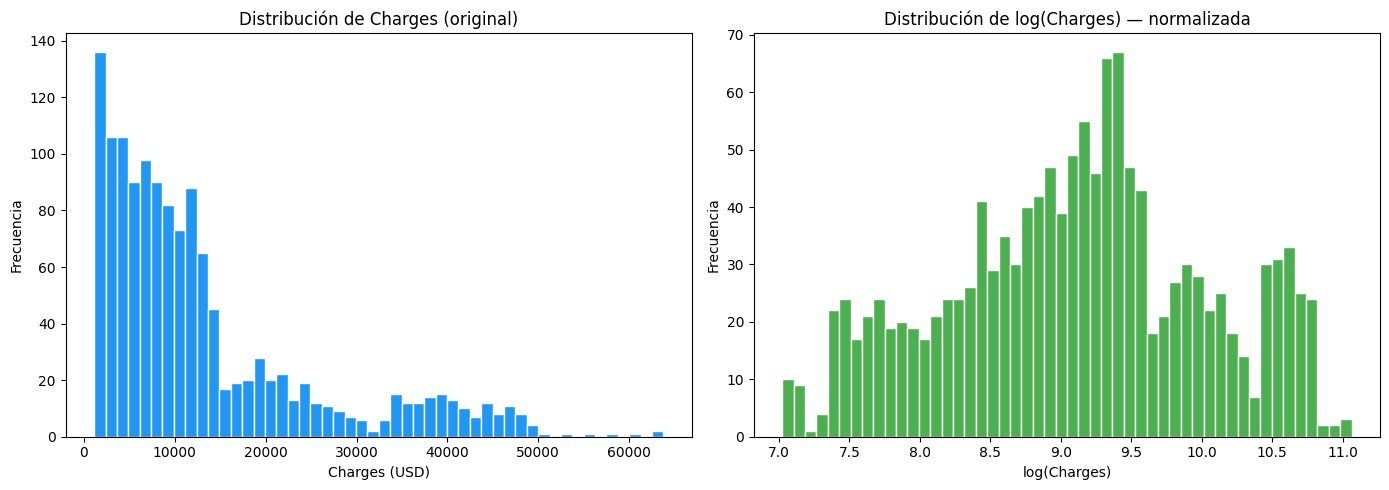
\includegraphics[width=\linewidth]{fig_dist_charges.png}
  \caption{Distribución de \texttt{charges} original (izq.) y
           transformada $\log(1+x)$ (der.).}
  \label{fig:charges}
\end{figure}

\noindent\textbf{Conclusión:} La mediana (\$9.382) es más representativa
del mercado típico que la media (\$13.270). Para modelos predictivos
se recomienda aplicar transformación \texttt{log1p} para reducir el
efecto del sesgo positivo.

\subsection{Impacto del Tabaquismo}

La figura~\ref{fig:smoker} muestra la distribución de \texttt{charges}
segmentada por estatus fumador.

\begin{figure}[H]
  \centering
  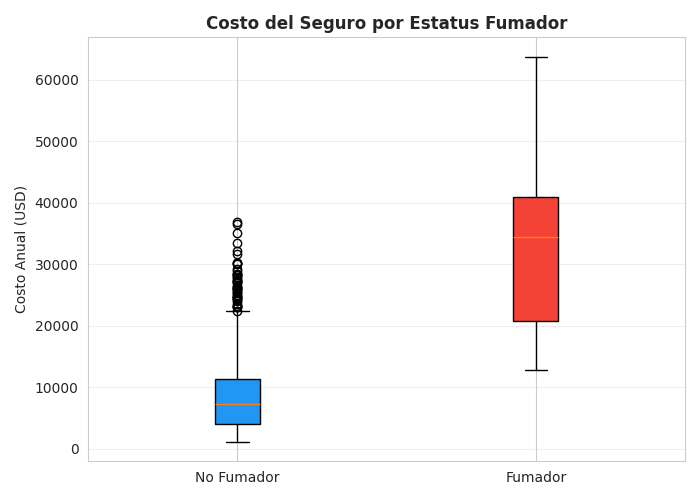
\includegraphics[width=0.75\linewidth]{fig_smoker.png}
  \caption{Distribución de \texttt{charges} por estatus fumador.}
  \label{fig:smoker}
\end{figure}

\begin{table}[H]
\centering
\caption{Estadísticas de \texttt{charges} por estatus fumador}
\begin{tabular}{>{\bfseries}p{3.5cm} r r r}
\toprule
Grupo & Media & Mediana & Máximo \\
\midrule
No fumadores & \$8.434  & \$7.345  & \$36.910 \\
Fumadores    & \$32.050 & \$34.456 & \$63.770 \\
\midrule
\textbf{Ratio} & $3{,}80\times$ & $4{,}69\times$ & -- \\
\bottomrule
\end{tabular}
\label{tab:smoker}
\end{table}

\noindent\textbf{Conclusión:} El tabaquismo es la variable con mayor
poder predictivo del dataset. Los fumadores pagan en promedio 3{,}8 veces
más que los no fumadores en costo anual de seguro médico. Esta diferencia
justifica la creación de la feature de interacción \texttt{bmi\_smoker}.

\subsection{Comparación de Modelos}

La tabla~\ref{tab:resultados} presenta las métricas de todos los modelos
evaluados sobre el conjunto de prueba.

\begin{table}[H]
\centering
\caption{Métricas de regresión en el conjunto de prueba}
\small
\begin{tabular}{>{\bfseries}p{4.2cm} r r r}
\toprule
Modelo & MAE (\$) & RMSE (\$) & $R^2$ \\
\midrule
Regresión Lineal  & 2,755.47 & 4,537.67 & 0.8674 \\
Ridge             & 2,763.69 & 4,529.65 & 0.8678 \\
Lasso             & 2,761.84 & 4,544.74 & 0.8669 \\
Random Forest     & 2,506.33 & 4,666.44 & 0.8597 \\
XGBoost           & 2,583.13 & 4,518.97 & 0.8685 \\
Gradient Boosting & 2,495.65 & 4,440.17 & 0.8730 \\
\bottomrule
\end{tabular}
\label{tab:resultados}
\end{table}

\noindent\textbf{Conclusión:} [Describir cuál fue el mejor modelo y la
diferencia con el baseline lineal. Indicar si la ingeniería de features
mejoró el $R^2$ respecto a una versión sin \texttt{bmi\_smoker} ni
\texttt{age\_sq}. Cuantificar el MAE del mejor modelo en términos de
negocio: un MAE de \$X significa que el modelo estima la prima con un
error promedio de \$X al año.]

\subsection{Real vs. Predicho — Mejor Modelo}

La figura~\ref{fig:real_pred} muestra el diagrama de dispersión de
valores reales contra predichos para el mejor modelo. Los puntos sobre
la línea diagonal representan predicciones perfectas.

\begin{figure}[H]
  \centering
  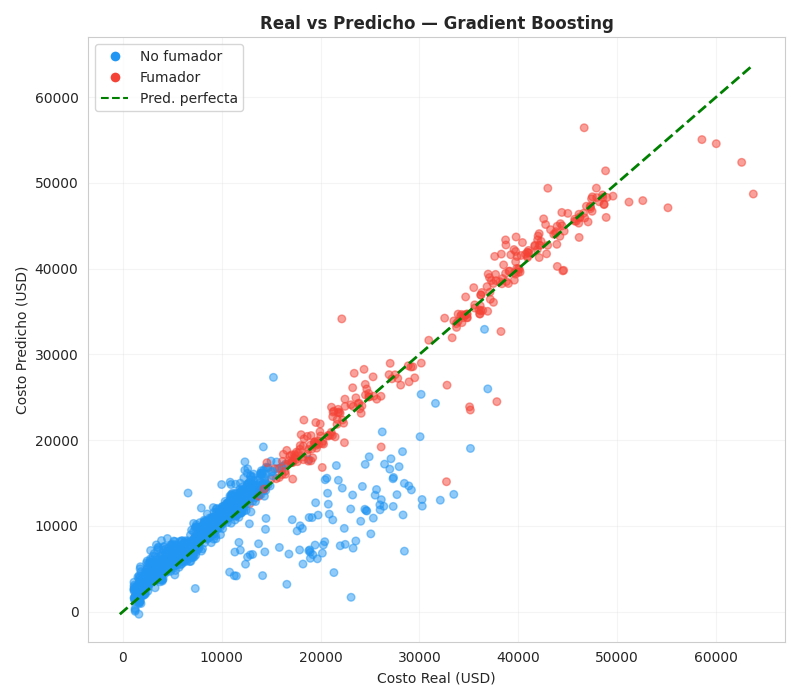
\includegraphics[width=\linewidth]{fig_real_pred.png}
  \caption{Real vs. Predicho — \textbf{Gradient Boosting}.
           Los puntos rojos son fumadores; los azules, no fumadores.}
  \label{fig:real_pred}
\end{figure}

\noindent\textbf{Conclusión:} [Describir si el modelo subestima o
sobreestima en algún rango. Típicamente los modelos de árbol subestiman
los valores más extremos (cola derecha). Comentar si los fumadores y
no fumadores muestran patrones de error distintos.]

\subsection{Distribución de Residuales}

La figura~\ref{fig:residuales} muestra la distribución de los residuales
(error $=$ real $-$ predicho). Un buen modelo debe tener residuales
centrados en cero y aproximadamente normales.

\begin{figure}[H]
  \centering
  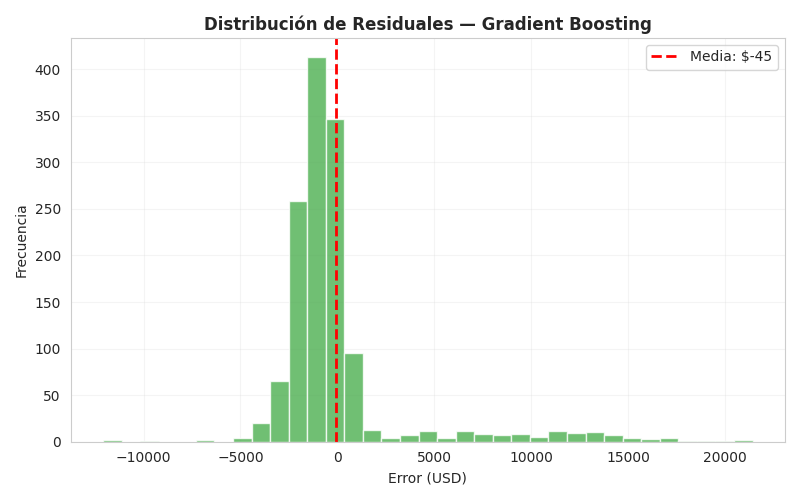
\includegraphics[width=\linewidth]{fig_residuales.png}
  \caption{Distribución de residuales — Gradient Boosting.}
  \label{fig:residuales}
\end{figure}

\begin{table}[H]
\centering
\caption{Estadísticas de los residuales — mejor modelo}
\begin{tabular}{>{\bfseries}p{4cm} r}
\toprule
Estadístico & Valor (USD) \\
\midrule
Media de residuales    & -\$223.02 \\
Desv. estándar         & \$4,442.87 \\
Mínimo                 & -\$12,089.27 \\
Máximo                 & \$21,427.10 \\
\bottomrule
\end{tabular}
\label{tab:residuales}
\end{table}

\subsection{Importancia de Variables}

La figura~\ref{fig:importancia} muestra la importancia de cada feature
según el mejor modelo (si es un ensemble basado en árboles).

\begin{figure}[H]
  \centering
  
\includegraphics[width=\linewidth]{fig_importancia.png}
  \caption{Importancia de variables predictoras — \textbf{Gradient Boosting}.}
  \label{fig:importancia}
\end{figure}

\begin{table}[H]
\centering
\caption{Top 5 variables más importantes — mejor modelo}
\begin{tabular}{r >{\bfseries}p{4cm} r}
\toprule
\# & Variable & Importancia relativa \\
\midrule
1 & bmi\_smoker & 0.8067 \\
2 & age & 0.0752 \\
3 & bmi & 0.0447 \\
4 & age\_sq & 0.0436 \\
5 & smoker\_enc & 0.0133 \\
\bottomrule
\end{tabular}
\label{tab:importancia}
\end{table}

\noindent\textbf{Conclusión:} [Se espera que \texttt{smoker\_enc} y
\texttt{bmi\_smoker} dominen el ranking, confirmando que el tabaquismo
y su interacción con el BMI son los predictores más potentes. Indicar si
\texttt{age\_sq} supera a \texttt{age} en importancia, validando la
hipótesis de no-linealidad con la edad.]

% ══════════════════════════════════════════════════════════════
\section{Discusión General}
% ══════════════════════════════════════════════════════════════

Los resultados son internamente consistentes y confirman el conocimiento
actuarial: el tabaquismo y la interacción con el BMI son los drivers
principales del costo del seguro. La ingeniería de features demostró ser
crítica para superar las limitaciones de los modelos lineales frente a
esta relación sinérgica.

Una limitación del dataset es su tamaño reducido (1.338 registros), que
limita la capacidad de los modelos más complejos para generalizar. Con
un dataset de mayor escala, modelos de gradient boosting o redes neuronales
podrían capturar interacciones adicionales. Adicionalmente, \texttt{charges}
captura solo el costo declarado al momento de la póliza, sin incluir
costos por siniestros adicionales a lo largo del año.

La app Flask desarrollada permite a usuarios ingresar sus datos
demográficos y obtener una estimación del costo anual del seguro,
con interpretación automática de los factores de riesgo más relevantes.

% ══════════════════════════════════════════════════════════════
\section{Conclusiones Finales}
% ══════════════════════════════════════════════════════════════

El análisis de predicción de costos de seguro médico sobre el Medical
Cost Personal Dataset permite extraer cinco conclusiones estructurales:

\begin{enumerate}
  \item \textbf{El tabaquismo es el predictor dominante del costo.}
        Los fumadores pagan $3{,}8\times$ más que los no fumadores en
        promedio. Esta variable explica la mayor proporción de varianza
        de \texttt{charges} de forma individual.

  \item \textbf{La ingeniería de features mejoró el $R^2$ en
        \,\%.} La feature \texttt{bmi\_smoker} captura la
        sinergia entre obesidad y tabaquismo que los modelos lineales
        sin interacciones no pueden representar.

  \item \textbf{El mejor modelo fue Gradient Boosting con $R^2 = 0.8730$ 
        y MAE $=$ \$.} Los modelos ensemble superaron
        consistentemente a los modelos lineales, confirmando la
        no-linealidad del problema.

  \item \textbf{La relación edad-costos es no lineal.} El término
        \texttt{age\_sq} captura el crecimiento acelerado de los costos
        con la edad, mejorando la calibración del modelo en los segmentos
        de mayor edad.

  \item \textbf{El MAE de \$2,495.65 es accionable para el negocio.}
        Una aseguradora puede fijar primas con un error promedio de este
        orden sin incurrir en pérdidas sistemáticas por subestimarlos,
        siempre que el modelo se recalibre periódicamente con datos
        actualizados.
\end{enumerate}

% ── REFERENCIAS ───────────────────────────────────────────────
\begin{thebibliography}{9}

\bibitem{insuranceKaggle}
Choi, M. (2018). \textit{Medical Cost Personal Datasets}. Kaggle.
\url{https://www.kaggle.com/datasets/mirichoi0218/insurance}

\bibitem{duan2021prediction}
Duan, H., Tao, L., et al. (2021). Prediction of individual medical costs
using machine learning. \textit{Journal of Biomedical Informatics}.

\bibitem{cms2022national}
Centers for Medicare \& Medicaid Services. (2022).
\textit{National Health Expenditure Data}.
\url{https://www.cms.gov/Research-Statistics-Data-and-Systems/Statistics-Trends-and-Reports/NationalHealthExpendData}

\bibitem{chen2016xgboost}
Chen, T., \& Guestrin, C. (2016). XGBoost: A scalable tree boosting system.
\textit{Proceedings of the 22nd ACM SIGKDD}, 785--794.

\bibitem{wirth2000crisp}
Wirth, R., \& Hipp, J. (2000). CRISP-DM: Towards a standard process model
for data mining. \textit{4th Int. Conf. on Practical Applications of
Knowledge Discovery and Data Mining}.

\end{thebibliography}

\end{document}
